\section{Kubernetes. Контейнерная виртуализация. Архитектура. Под.}


\D{
    Контейнер - легковесный пакет кода приложения со всеми необходимыми
    зависимостями (библиотеки, окружение).

    Контейнерная виртуализация позволяет совместно использовать
    ресурсы на уровне ОС.
}

\begin{figure}[H]
	\centering
	\begin{minipage}[b]{0.8\textwidth}
		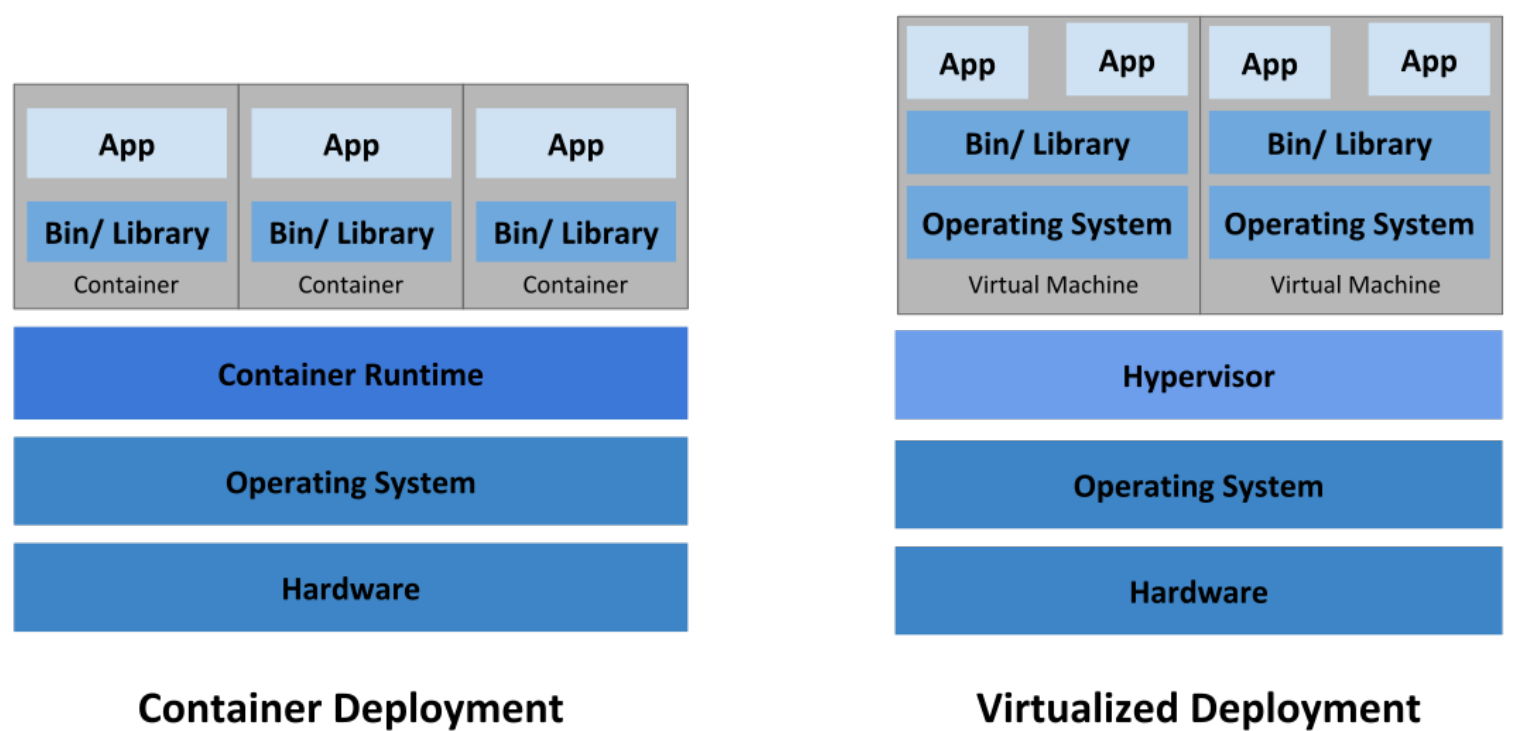
\includegraphics[width=\textwidth]{images/cdep.png}
	\end{minipage}
\end{figure}

\textbf{Docker} - платформа контейнерной виртуализации.

\subsection*{Kubernetes}

\D{
    Kubernetes - решение для оркестрации контейнеров.
}

Архитектура:
\begin{itemize}
    \item ApiServer
    \item etcd
    \item Scheduler
    \item Kube-Controller
    \item Kubelet
    \item Kube-Proxy
\end{itemize}

\begin{figure}[H]
	\centering
	\begin{minipage}[b]{0.8\textwidth}
		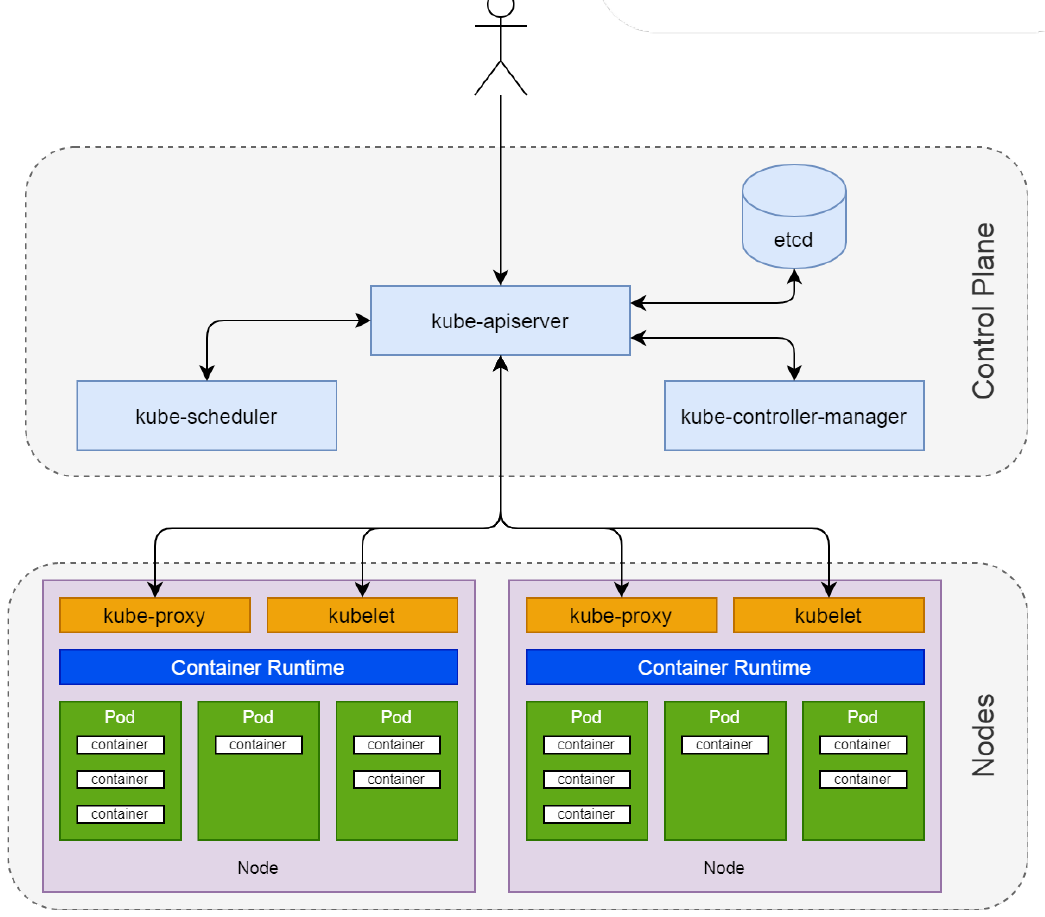
\includegraphics[width=\textwidth]{images/kuba.png}
        \caption{Kubernetes architecture}
	\end{minipage}
\end{figure}

\D{
    Pod - наименьшая развертываемая единица Kubernetes.

    Pod состоит из одного или более контейнеров.

    Все контейнеры запускаются на одной машине.
}

\textbf{kubectl} - утилита для управления подами.